\documentclass[main.tex]{subfiles}

\begin{document}

	\begingroup

	\renewcommand{\cleardoublepage}{}

	\renewcommand{\clearpage}{}

	\chapter{Knowledge Function Documentation}

		\chapterauthor{Jeremias Thun}

All the Information about the existing surfaces and the objects are managed in our Knowledgebase. Every question about the relationship between these Objects as well as which one should be taken next and where should it be put is answerd by this Knowledgebase.  The Knowledgebase is built as part of KnowRob. All data is stored as RDF triple, organized by an OWL ontology. This is where logical relationship between the category of objects and surfaces is implemented. \\
		
\section{Knowledge base}
\chapterauthor{Jeremias Thun}

The Knowledge base as well as knowrob is written in Prolog. To interact manually with the knowledge base, you can (after you started Knowledge) run
\begin{lstlisting}
rosrun rosprolog rosprolog_commandline.py
\end{lstlisting}
which opens a prolog shell in your commandline.

\subsection{object\_state.pl}

First of all, we need to add some objects that we can work on to our Knowledgebase. This is where the perceived objects go when the Percpetion-Group found something:

\begin{lstlisting}
create_object_at(
	PerceivedObjectType, 
	PercTypeConfidence, 
	Transform, 
	Threshold, 
	Instance, 
	[Width, Depth, Height], 
	Shape, 
	PercShapeConfidence, 
	Color, 
	PercColorCondidence) :-
\end{lstlisting}
This confusingly big predicate takes all the perceived Data, creates a corresponding Object in the Knowledgebase and adds all the attributes. Within this procedure, there are a few verifications and changes made, though: The Class, Shape and Color of the Object all have a probability with which they are correctly perceived. These confidences are stored as link to the Object (more on that in the OWL-Chapter), but only if they satisfy a secified threshold. If they don't, the attributes are set back to default values. Also we check if the given data makes any sence, i.e. if the object has a reasonable size.\\
Besides a few helper predicates, this module also contains two helpful little predicates to get all Objects that are stored at that moment:
\begin{lstlisting}
hsr_existing_objects(Objects) :-
    belief_existing_objects(Objects, [hsr_objects:'Item']).
\end{lstlisting}
And there \texttt{hsr\_forget\_object/1} removes an Object from the beliefstate:
\begin{lstlisting}
hsr_forget_object(Object) :-
    rdf_retractall(Object,_,_).
\end{lstlisting}

\subsection{beliefstate.pl}

In the Belief State mostly all changing information about our Knowledge is managed. Here lie the predicates that are called in \texttt{create\_object\_at/9}. To actually create a new Object in our belief state, there is:
\begin{lstlisting}
new_perceived_at(ObjType, Transform, Threshold, Instance) :-
\begin{lstlisting}
This Module also gives the opportunity to look at a specific Position in the map and ask, whether there already is a known Object and, if so, which one:
\begin{lstlisting}
hsr_existing_object_at(_, Transform, Threshold, Instance) :-
\end{lstlisting}
To determine, whether an object is hard to grasp it is often helpful to know, whether there are other objects right next to it. That is why there is a specific attribute that stores Groups of Objectts. 
\begin{lstlisting}
group_objects(Objs)
\end{lstlisting}
This Predicate takes a list of Objects and iterates through them to see if there are any groups and create them if necessary.\\
To make it more human-readable, there are also two other predicates that basically just call \texttt{group\_objects} with a different list of Objects:
\begin{lstlisting}
group_shelf_objects/0
group_table_objects/0
\end{lstlisting}

\subsubsection{Finding a surface}\label{sec:kn_find_surf}

The second part of our beliefstate decides, what surface Knowledge beliefs to be the most fit for an object at a certain time. This part still has a few flaws but here is what it can do:\\
When 

\subsection{pickup.pl}

In the pickup module the information necessary to pick an object up are organized.

\begin{lstlisting}
next_object_(BestObj) :-
\end{lstlisting}
As soon as there are some objects stored in our beliefstate, Knowledge is able zu tell, which Object should be the next one, the robot takes and puts somewhere. This prediacte returns the Object, that is standing on a surface, that was previously declared as \texttt{source} surface and is closest to the robot.

\subsection{assignplaces.pl}

Like \texttt{pickup.pl}, this module organizes the information necessary for when an object is placed.\\

In the end, everything Planning needs is given by
\begin{lstlisting}
object_goal_pose_offset_(Instance, [[X,Y,Z], Rotation],Context):-
\end{lstlisting}
It takes an Object and returns the pose this object should be placed in and as Context it also returns, why this decision was made the way it was.\\
But this predicate actually contains a few other queries. Some of the most important ones are:

\begin{lstlisting}
object_goal_surface_(Instance, NearestSurface, Context, Self) :-
\end{lstlisting}
First we need a decision about what surface the object should be placed on. This is simply based on which surface is nearest to the robot and has the attribute of a \texttt{target} surface.
\begin{lstlisting}
most_related_object(Source, Target, Distance) :-
distance_to_object(Source, Target, Distance) :-
\end{lstlisting}

 Here lies the decision about what object is most similar to the one, \texttt{object\_goal\_pose\_offset} got. \texttt{distance\_to\_object} can tell, how similar two objects are (what the legical distance between them is) in the class hierarchy. This is based on the knowrob-predicate \texttt{distance\_of/3}. The \texttt{most\_related\_obeject} iterates through every object already in place and either finds a similar one based on similar object-classes or, in case the class of our object is \texttt{Other}, looks for another object that has the same color or size as our object. This is also, where the context, i.e. the human readable reason why the object was placed the way it was, is generated. It tells us, if the decision was based on it's class (if so, how similar they were), on it's size or it's color.

\subsection{surfaces.pl}

The bigges module is the \texttt{surfaces} module. This is where you can find everything you need to know about surfaces.\\
The surfaces are, just like objects, stored as an atom, wich represents an instance of an OWL-Class and look like this:
\begin{lstlisting}
?- is_surface('http://ontologydesignpatterns.org/ont/dul/DUL.owl#PhysicalObject_UHOJSVEC')
true.
\end{lstlisting}
The only exception is the surface \texttt{ground}, which has no representation in the URDF, and is just an infinite surface that is everywhere below a certain height. This surface is just stored like this:
\begin{lstlisting}
?- is_surface(ground)
true.
\end{lstlisting}

\subsubsection{find surfaces}

You can call
\begin{lstlisting}
all_surfaces/1
\end{lstlisting}
to get all surfaces that are loaded in the URDF regardless of their role of if they even have a role. This predicate comes in handy, if you want to iterate through the available surfaces.\\
To find surfaces of a specific type, there are equivilent predicates that can give you lists of all tables, shelves, the ground or all source or target surfaces:
\begin{lstlisting}
all_source_surfaces/1
all_target_surfaces/1
ground_surface/1
shelf_surfaces/1
table_surfaces/1
\end{lstlisting}

There are also a few predicates that go in the other direction: If you have a surface and want to know if it is of a certain type, you can execute one of the following predicates:
\begin{lstlisting}
surface_type_of(Surrface, Type) :-

is_surface(Surface) :-
    all_surfaces(Surfaces),
    member(Surface, Surfaces).

is_table(Table) :-
    table_surfaces(Tables),
    member(Table, Tables).

is_shelf(Shelf) :-
    shelf_surfaces(Shelves),
    member(Shelf, Shelves).
\end{lstlisting}
\texttt{surface\_type\_of/2} expects returns the type as simple atom, which can be \texttt{ground}, \texttt{table} or \texttt{shelf}.\\
Last but not least there is 
\begin{lstlisting}
find_supporting_surface/2
\end{lstlisting}
which goes in both directions and links an object to the surface it is standing on.

\subsubsection{Get poses}
When the Roboter first goes to a surface to scan the objects that are standing there, Planning need to know the positions of those surfaces. That's what this chapter is about. It is based on
\begin{lstlisting}
pose_of_surfaces(Surfaces, Positions) :-
\end{lstlisting}
which takes a list of surfaces, sorts them by their distance to the roboter (where the nearest surface comes first in the list) and returns the sorted list of their positions.\\
The two other predicates just call \texttt{pose\_of\_surfaces/2} with a preset list of surfaces of a specified type:
\begin{lstlisting}
pose_of_tables(Positions) :-
pose_of_shelves(Positions) :-
\end{lstlisting}

\subsubsection{Find Objects}
As an equivilant to \texttt{is\_surface} we also have
\begin{lstlisting}
is_object/1
\end{lstlisting}
To find Objects, there is our core predicate
\begin{lstlisting}
objects_on_list_of_surfaces(ObjectInstances, SurfaceList):-
\end{lstlisting}
which just runs through all the given surfaces and returns a list of every object that was found on them.\\
All the other predicates in this chapter are variations of this idea:
\begin{lstlisting}
objects_on_surface/2,
all_objects_on_source_surfaces/1,
all_objects_on_target_surfaces/1,
all_objects_on_ground/1,
all_objects_in_whole_shelf_/1,
all_objects_on_tables_/1,
\end{lstlisting}

\subsubsection{Roles}

\begin{figure}
    \centering
    %\begin{minipage}{0.45\textwidth}
    %    \centering
        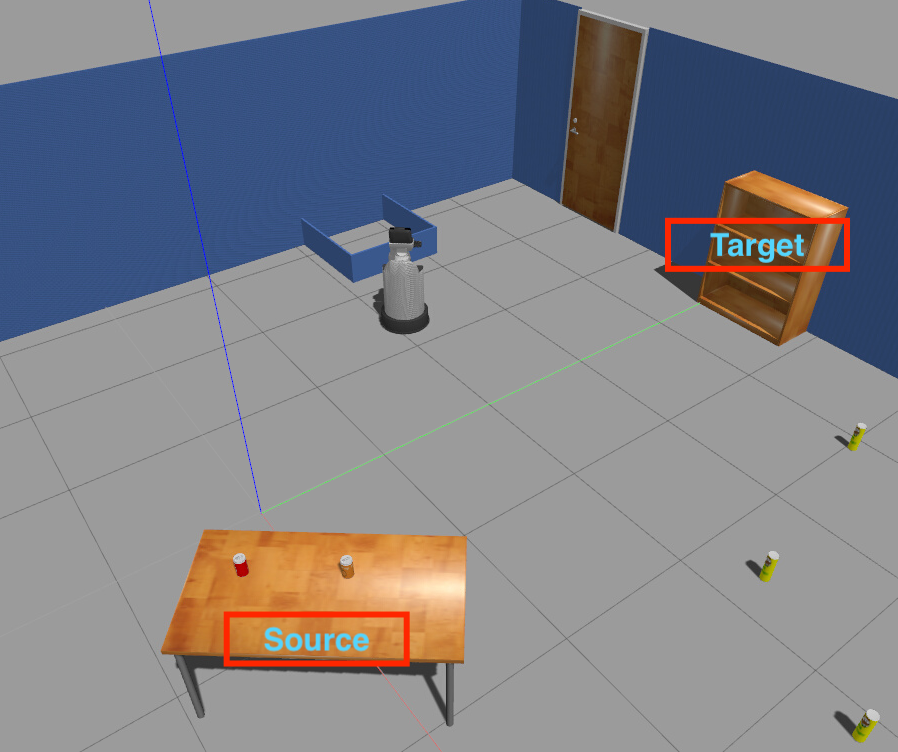
\includegraphics[width=0.8\textwidth]{pictures/knowledge_roles_gr.png}
        \caption{Roles in Grocery Storing}
        \label{fig:kn_ro_gr}
    %\end{minipage}\hfill
    %\begin{minipage}{0.45\textwidth}
        \centering
        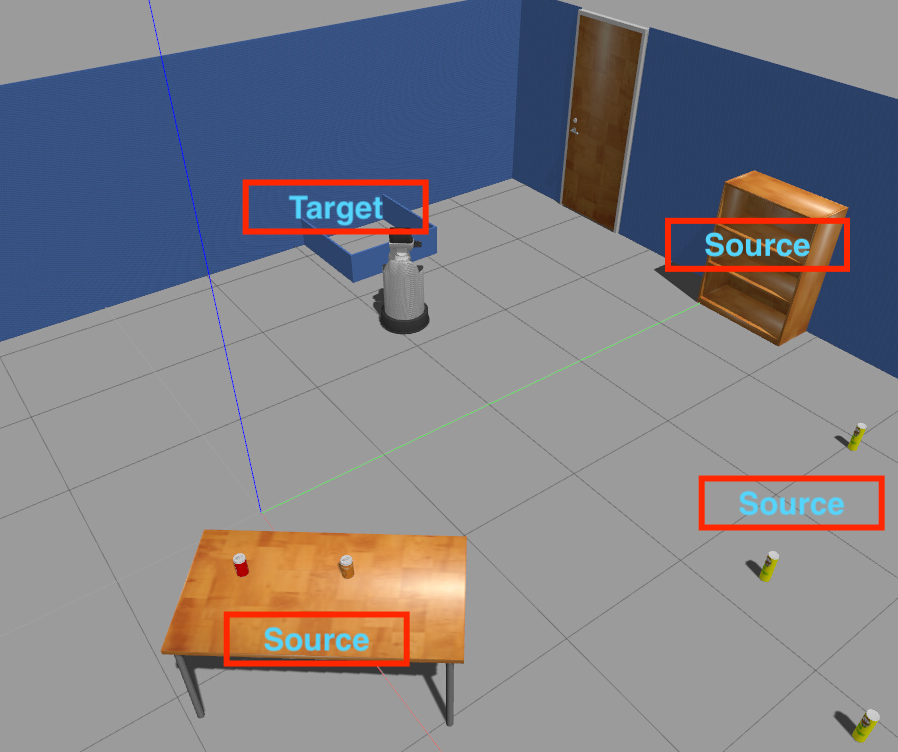
\includegraphics[width=0.8\textwidth]{pictures/knowledge_roles_cl.png}
        \caption{Roles in Clean Up}
        \label{fig:kn_ro_cl}
    %\end{minipage}
\end{figure}

To be able to use the same predicates for both Tasks Grocery Storing and Cleanup, we implemented the concept of a surface role. All the most important predicates do something at a surface, depending on it's role. For example, when we find the next object to grasp, it should be the next object standing on a surface, that we want to grasp from. Or when we place an object on a surface, it should be a surface that we want to put things on. Which surfaces get what role only depends on the task that the robot is currently working on. In the Grocery Storing task, all the shelves are target surfaces and all the tables are source surfaces (see figure \ref{fig:kn_ro_gr}), in the Cleanup task only the basket is a target surfaces and everything else (including the ground) is a source surface (see figure \ref{fig:kn_ro_cl}). This way, knowledge doesn't need to know the specific task, it just needs to know, which surfaces have what role.\\
This is implemented by 

\begin{lstlisting}
make_role(SurfaceLink, Role):-
    rdf_retractall(SurfaceLink, hsr_objects:'sourceOrTarget',_),
    rdf_assert(SurfaceLink, hsr_objects:'sourceOrTarget', Role).
\end{lstlisting}
and there are a few other predicates, that use this \texttt{make\_role/2} and apply it to different lists of surfaces:
\begin{lstlisting}
% Gives a list of surfaces the role source
make_surfaces_source(Surfaces):-

% Gives a list of surfaces the role target
make_surfaces_target(Surfaces):-

% Gives all surfaces with given name (ground, table, basket or shelf) the Role (target or source)
make_all_surface_type_role(SurfaceType, Role):-
\end{lstlisting}


\subsection{spatial\_comp.pl}



\section{Ontology}
\chapterauthor{Fabian Rosenstock}
\subsection{About Ontologies}
An Ontology is a knowledge represantation. To fullfill this task ontologies define classes, their attributes and relations between them. Ontologies are hierarchical build and differnt axioms and restrictions for classes can be defined.


\subsection{Robocup}
The Robocup Ontology defines Concepts used to describe the Robocup and Concepts needed for the URDFs. To do that it imports the srdl2-comp ontology that is part of knowrob. Furthermore our objects ontology gets imported.\\


\subsection{Objects}

This Ontology describes and categorizes different physical objects according to their properties or common uses. These categories help to reason over objects, for example find similar objects. The Ontology furthermore defines different properties objects can have. \\
The objects ontology imports the knowrob and the urdf ontology provided by knowrob.\\
For the description of objects different regions are defined. Classes that represent different colors are added in the objects ontology as subclasses of ColorRegion and different materials are defined in subclasses of MaterialRegion. Different shapes are represented by subclasses of ShapeRegion.\\
For those characteristics subclasses of PhysicalQuality are added. Those represent the quality of the object, while the regions represent the actual values.\\
To represent the confidence with which the robot perceived a characteristic of an object the class ConfidenceRegion and subclasses for the different characteristics are defined.\\
The physical objects, we can encounter are represented by the subclasses of PhysicalObject.
One of these subclasses is PhysicalPlace. The subclasses of PhysicalPlace represent places, like the shelf. The surfaces are represented by subclasses of PhysicalPlace aswell. To represent these PhysicalPlace has the subclass Surface, where different kinds of surfaces are defined.\\
The Unknown class represents perceived objects, for which the robot doesnt know or is not sure what kind of physical object it is.\\
Most of the items, that have a representation in our ontology, are subclasses of DesignedArtifact.
Here you can find every item, that is created following a certain design. 
Examples for this are DesignedFurniture like a table and DesignedTools like a knife.\\
A huge part of the known items are different kinds of food or drinks. Most of these are categorised as ProcessedFood or Drink. Both of these are a subclass of DesignedSubstance. The exception to this are things like tomatoes, since these are not designed and therefor dont fit in the DesignedArtifact class. Those objects are categorised as NaturalFood, a subclass of BiologicalObject. This class is a subclass of PhysicalBody.\\
The object properties hassurface and issurfaceof are used to connect a surface and the dedicated object.\\
Since these surfaces can fullfill different roles the properties hasLocationRole and isLocationRoleOf are defined to connect the Source and Target roles to surfaces.\\
For the grouping of objects the property inGroup is responsible. This property connects an object to a group.\\
The supportedBy property connects an object to the object (most likely surface) it is standing on.\\
To store the confidence for the different characteristics subproperties of the property hasRegionDataValue have been added.\\
The size property is responsible for storing the size of an object.\\
To distinguish objects we can move from others we added the supportable property. This property stores a boolean for an object.



\section{Scripts and higher Architecture}
\chapterauthor{Fabian Rosenstock}	  	
\subsection{store\_object\_info\_server.py}
This script stores the send data in our Knowledge base.
To do that it first checks if the class name is empty. Furthermore the script changes the name of the class if it is not empty, since we have different naming conventions. After that it tests whether the class exists in our Ontology. If the classname is empty or if the class does not exist in our ontology the class gets changed to the generic other class. Then all the information on the object get extracted out of the ObjectDetectionData message. If the object has a legal position it gets added to the knowledge base and the objects at that position are put into one group.

	\endgroup

\end{document}
